%%%%%%%%%%%%%%%%%%%%%%%%%%%%%%%%%%%%%%%%%
% NIWeek 2014 Poster by T. Reveyrand
% www.microwave.fr
% http://www.microwave.fr/LaTeX.html
% ---------------------------------------
% 
% Original template created by:
% Brian Amberg (baposter@brian-amberg.de)
%
% This template has been downloaded from:
% http://www.LaTeXTemplates.com
%
% License:
% CC BY-NC-SA 3.0 (http://creativecommons.org/licenses/by-nc-sa/3.0/)
%
%%%%%%%%%%%%%%%%%%%%%%%%%%%%%%%%%%%%%%%%%

%----------------------------------------------------------------------------------------
%	PACKAGES AND OTHER DOCUMENT CONFIGURATIONS
%----------------------------------------------------------------------------------------

\documentclass[a0paper,portrait]{baposter}

\usepackage[font=small,labelfont=bf]{caption} % Required for specifying captions to tables and figures
\usepackage{booktabs} % Horizontal rules in tables
\usepackage{relsize} % Used for making text smaller in some places

\usepackage{amsmath,amsfonts,amssymb,amsthm} % Math packages
\usepackage{eqparbox}
\usepackage{fancybox}
\usepackage{textcomp}
\usepackage{multicol}
\usepackage{wrapfig} % Allows wrapping text around tables and figures

\graphicspath{{figures/}} % Directory in which figures are stored

 \definecolor{bordercol}{RGB}{40,40,40} % Border color of content boxes
 \definecolor{headercol1}{RGB}{186,215,230} % Background color for the header in the content boxes (left side)
 \definecolor{headercol2}{RGB}{120,120,120} % Background color for the header in the content boxes (right side)
 \definecolor{headerfontcol}{RGB}{0,0,0} % Text color for the header text in the content boxes
 \definecolor{boxcolor}{RGB}{186,228,188} % Background color for the content in the content boxes

\makeatletter 
\renewcommand{\baposter@box@drawbackground@plain}[2]{\tikzset{box colors/.style={fill=#1,fill opacity=0.8}} \fill[box colors] \baposterBoxGetShape;}
\makeatother

\begin{document}

\background{ % Set the background to an image (background.pdf)
\begin{tikzpicture}[remember picture,overlay]
\draw (current page.north west)+(+1em,-1em) node[anchor=north west]
{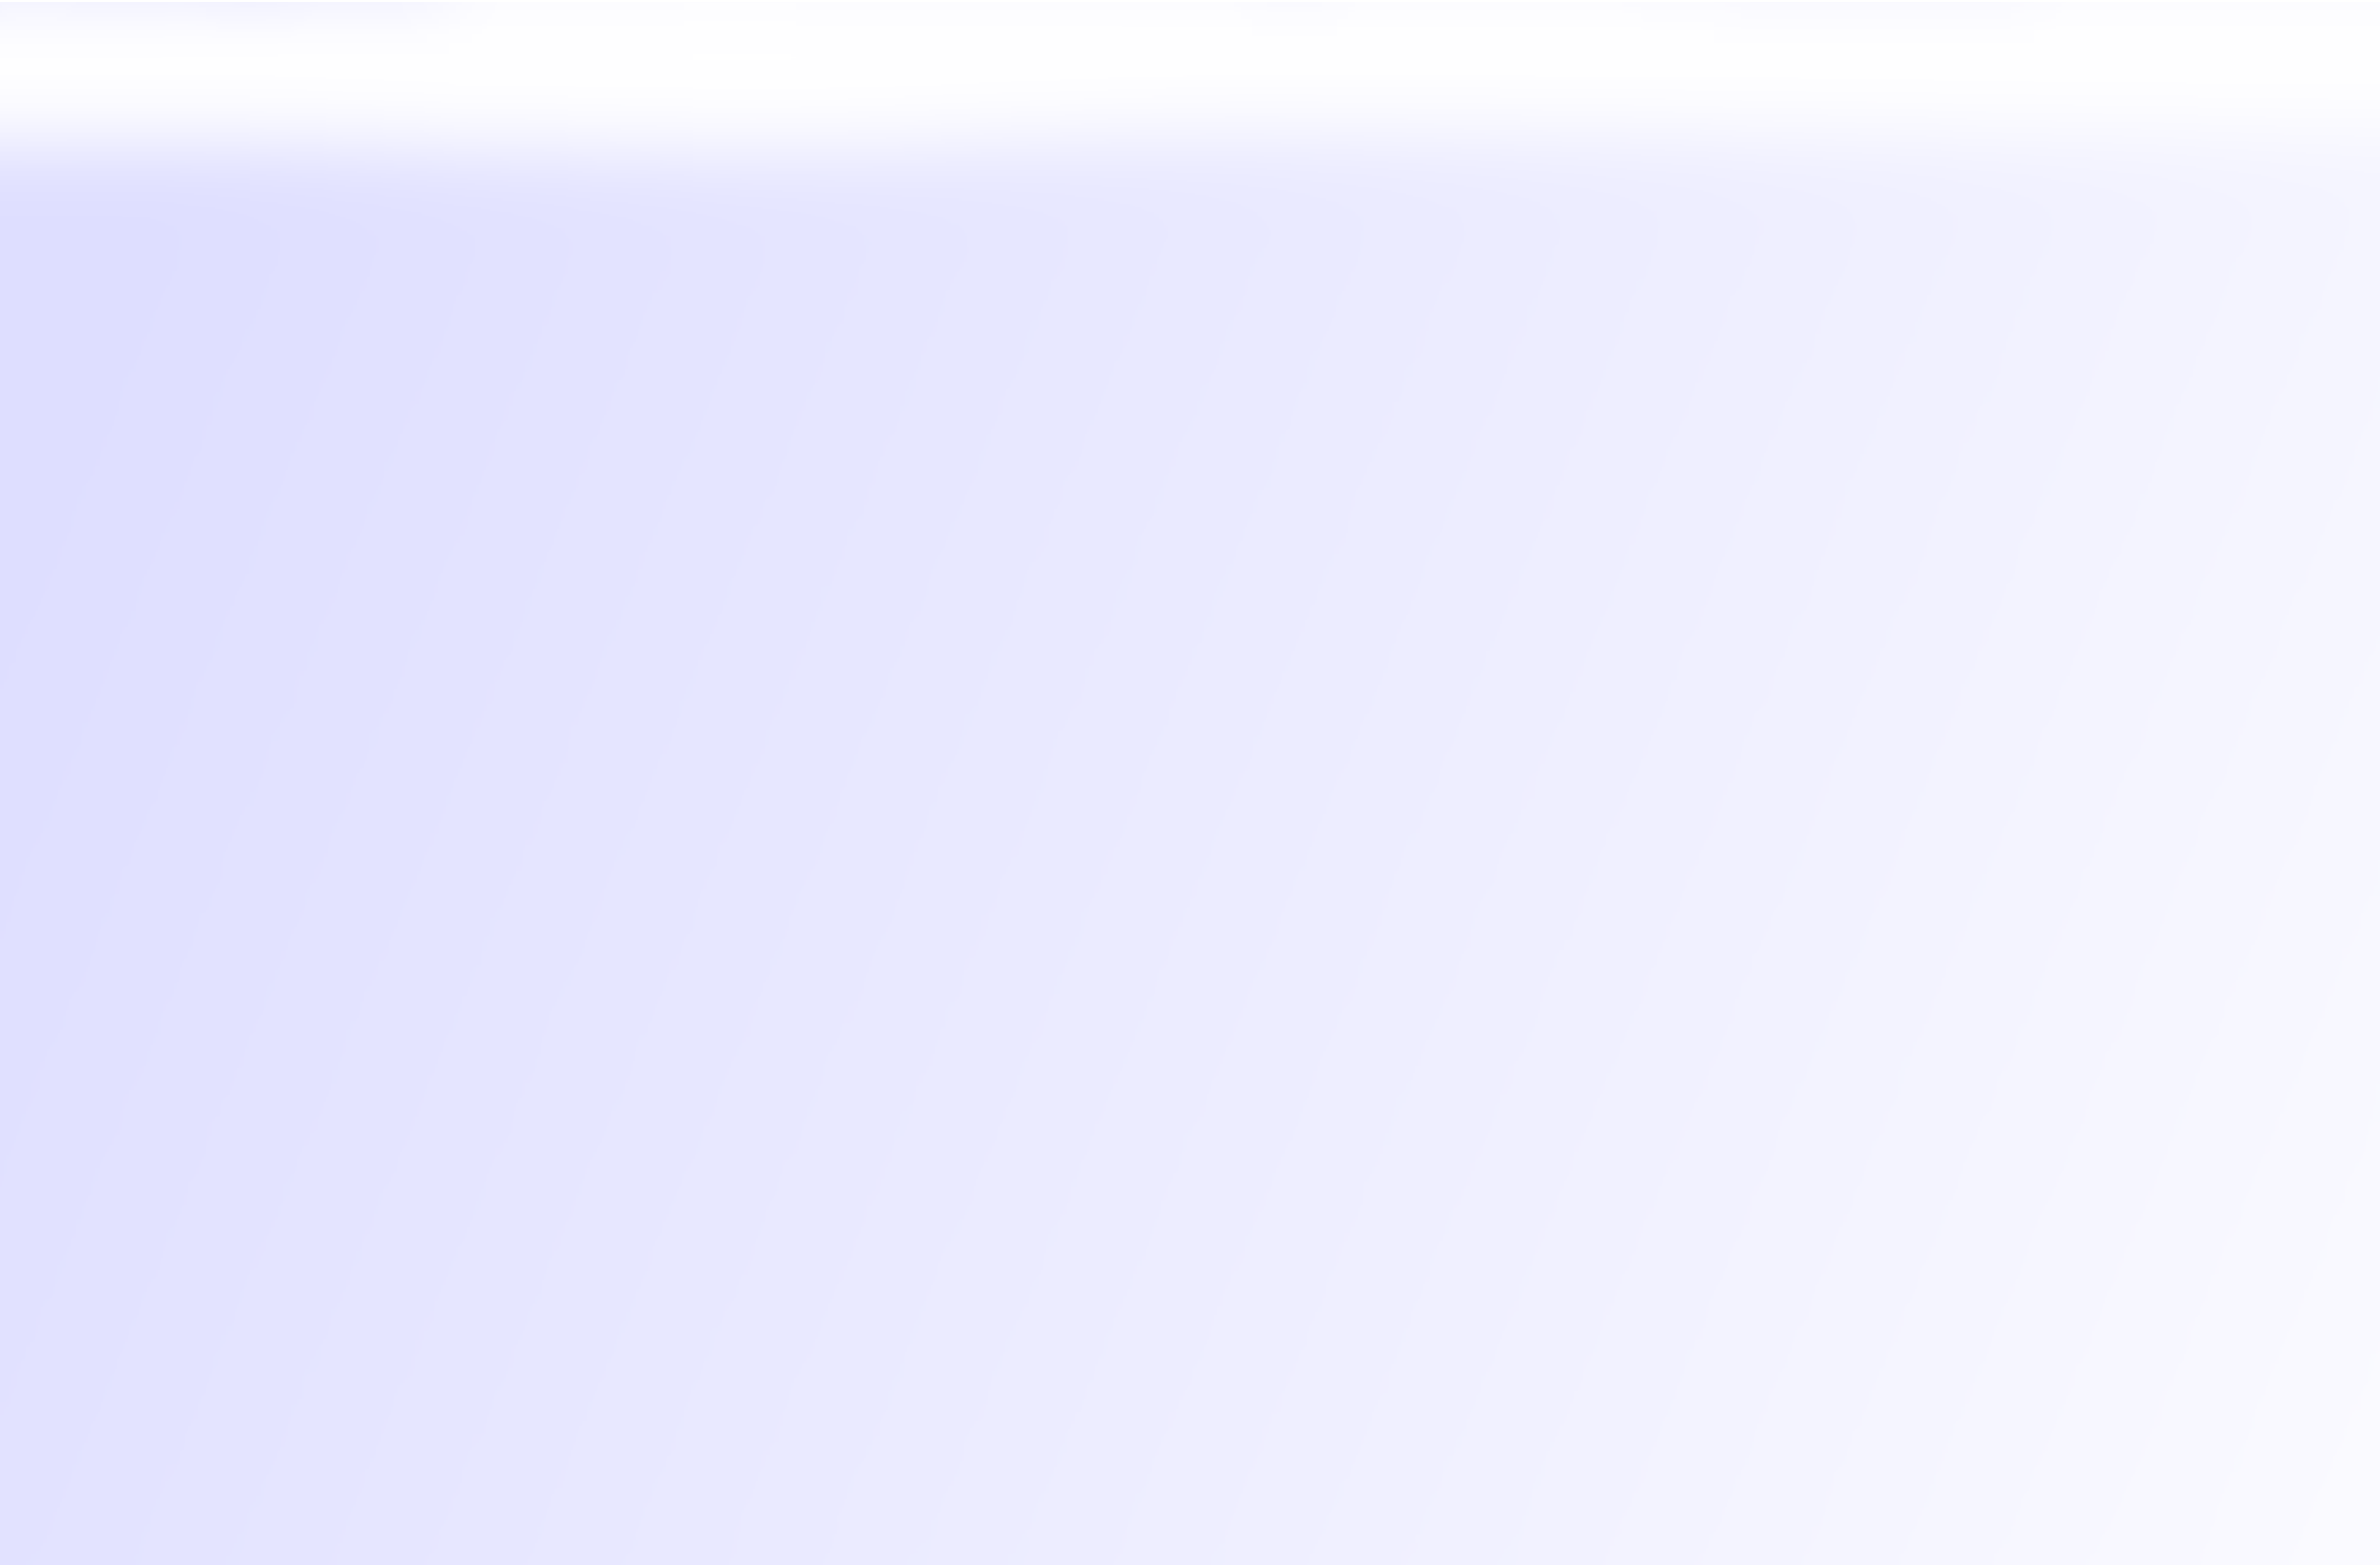
\includegraphics[height=0.5\textheight]{background.pdf}};
\end{tikzpicture}
}

\begin{poster}{
columns=2,
grid=false,
borderColor=bordercol, % Border color of content boxes
headerColorOne=headercol1, % Background color for the header in the content boxes (left side)
headerColorTwo=headercol2, % Background color for the header in the content boxes (right side)
headerFontColor=headerfontcol, % Text color for the header text in the content boxes
boxColorOne=white, % Background color for the content in the content boxes
headershape=roundedright, % Specify the rounded corner in the content box headers
headerfont=\Large\sf\bf, % Font modifiers for the text in the content box headers
textborder=rectangle,
background=user,
headerborder=open, % Change to closed for a line under the content box headers
boxshade=plain
}
{
\includegraphics[scale=0.18]{unach.png}}
%
%----------------------------------------------------------------------------------------
%	TITLE AND AUTHOR NAME
%----------------------------------------------------------------------------------------
%
{ \bf  \LARGE {Mobility for spheres using
MCT-HI's whit HNC Approximation
} }
%\Large \it A} % Poster title
{\vspace{0.3em} \small\sf Fidencio P\'erez Hern\'andez, Claudio Contreras Aburto\\  % Author names
\vspace{0.3em}
\small\sf { Facultad de Ciencias en F\'isica y Matem\'aticas, Universidad Aut\'onoma de Chiapas}\\
\vspace{0.3em}
\small\sf { Carretera Emiliano Zapata Km. 8, Ciudad Universitaria, 29050 Tuxtla Guti\'errez, Chiapas, M\'exico}} % Author email addresses
{
\includegraphics[scale=0.28]{LogoFCFM.jpg}} % University/lab logo

%----------------------------------------------------------------------------------------
%	ABSTRACT
%----------------------------------------------------------------------------------------
\headerbox{\small Abstract}{name=abstract,column=0,row=0, span=2,boxColorOne=green!30}{
\small{The electrophoretic mobility is the response function that describes the velocity of cherged particles in solutions, for this, in this study we have focused on studying salt molecules using MCT-HI's as a theoretical framework. In the other hand to get the correlation functions we have used the HNC approximation for the electrolyte solution. As a consequence of this study, conductivity can also be obtained and compared with experimental results. 
} % the cross-correlation analysis between high energies and radio emission, towards an estimate for the location of the high energy emission region. 
}
%----------------------------------------------------------------------------------------
%	OTHER INSTRUMENTATION
%----------------------------------------------------------------------------------------
\headerbox{\small Mobility in different salts (NaCl,...)}{name=instruments,column=1,row=1,span=1,below=abstract,boxColorOne=white!1}
{
\begin{center}
\noindent\shadowbox{\begin{minipage}[t]{1\textwidth - 2\fboxsep - 2\fboxrule - 2\shadowsize}%
{\centering
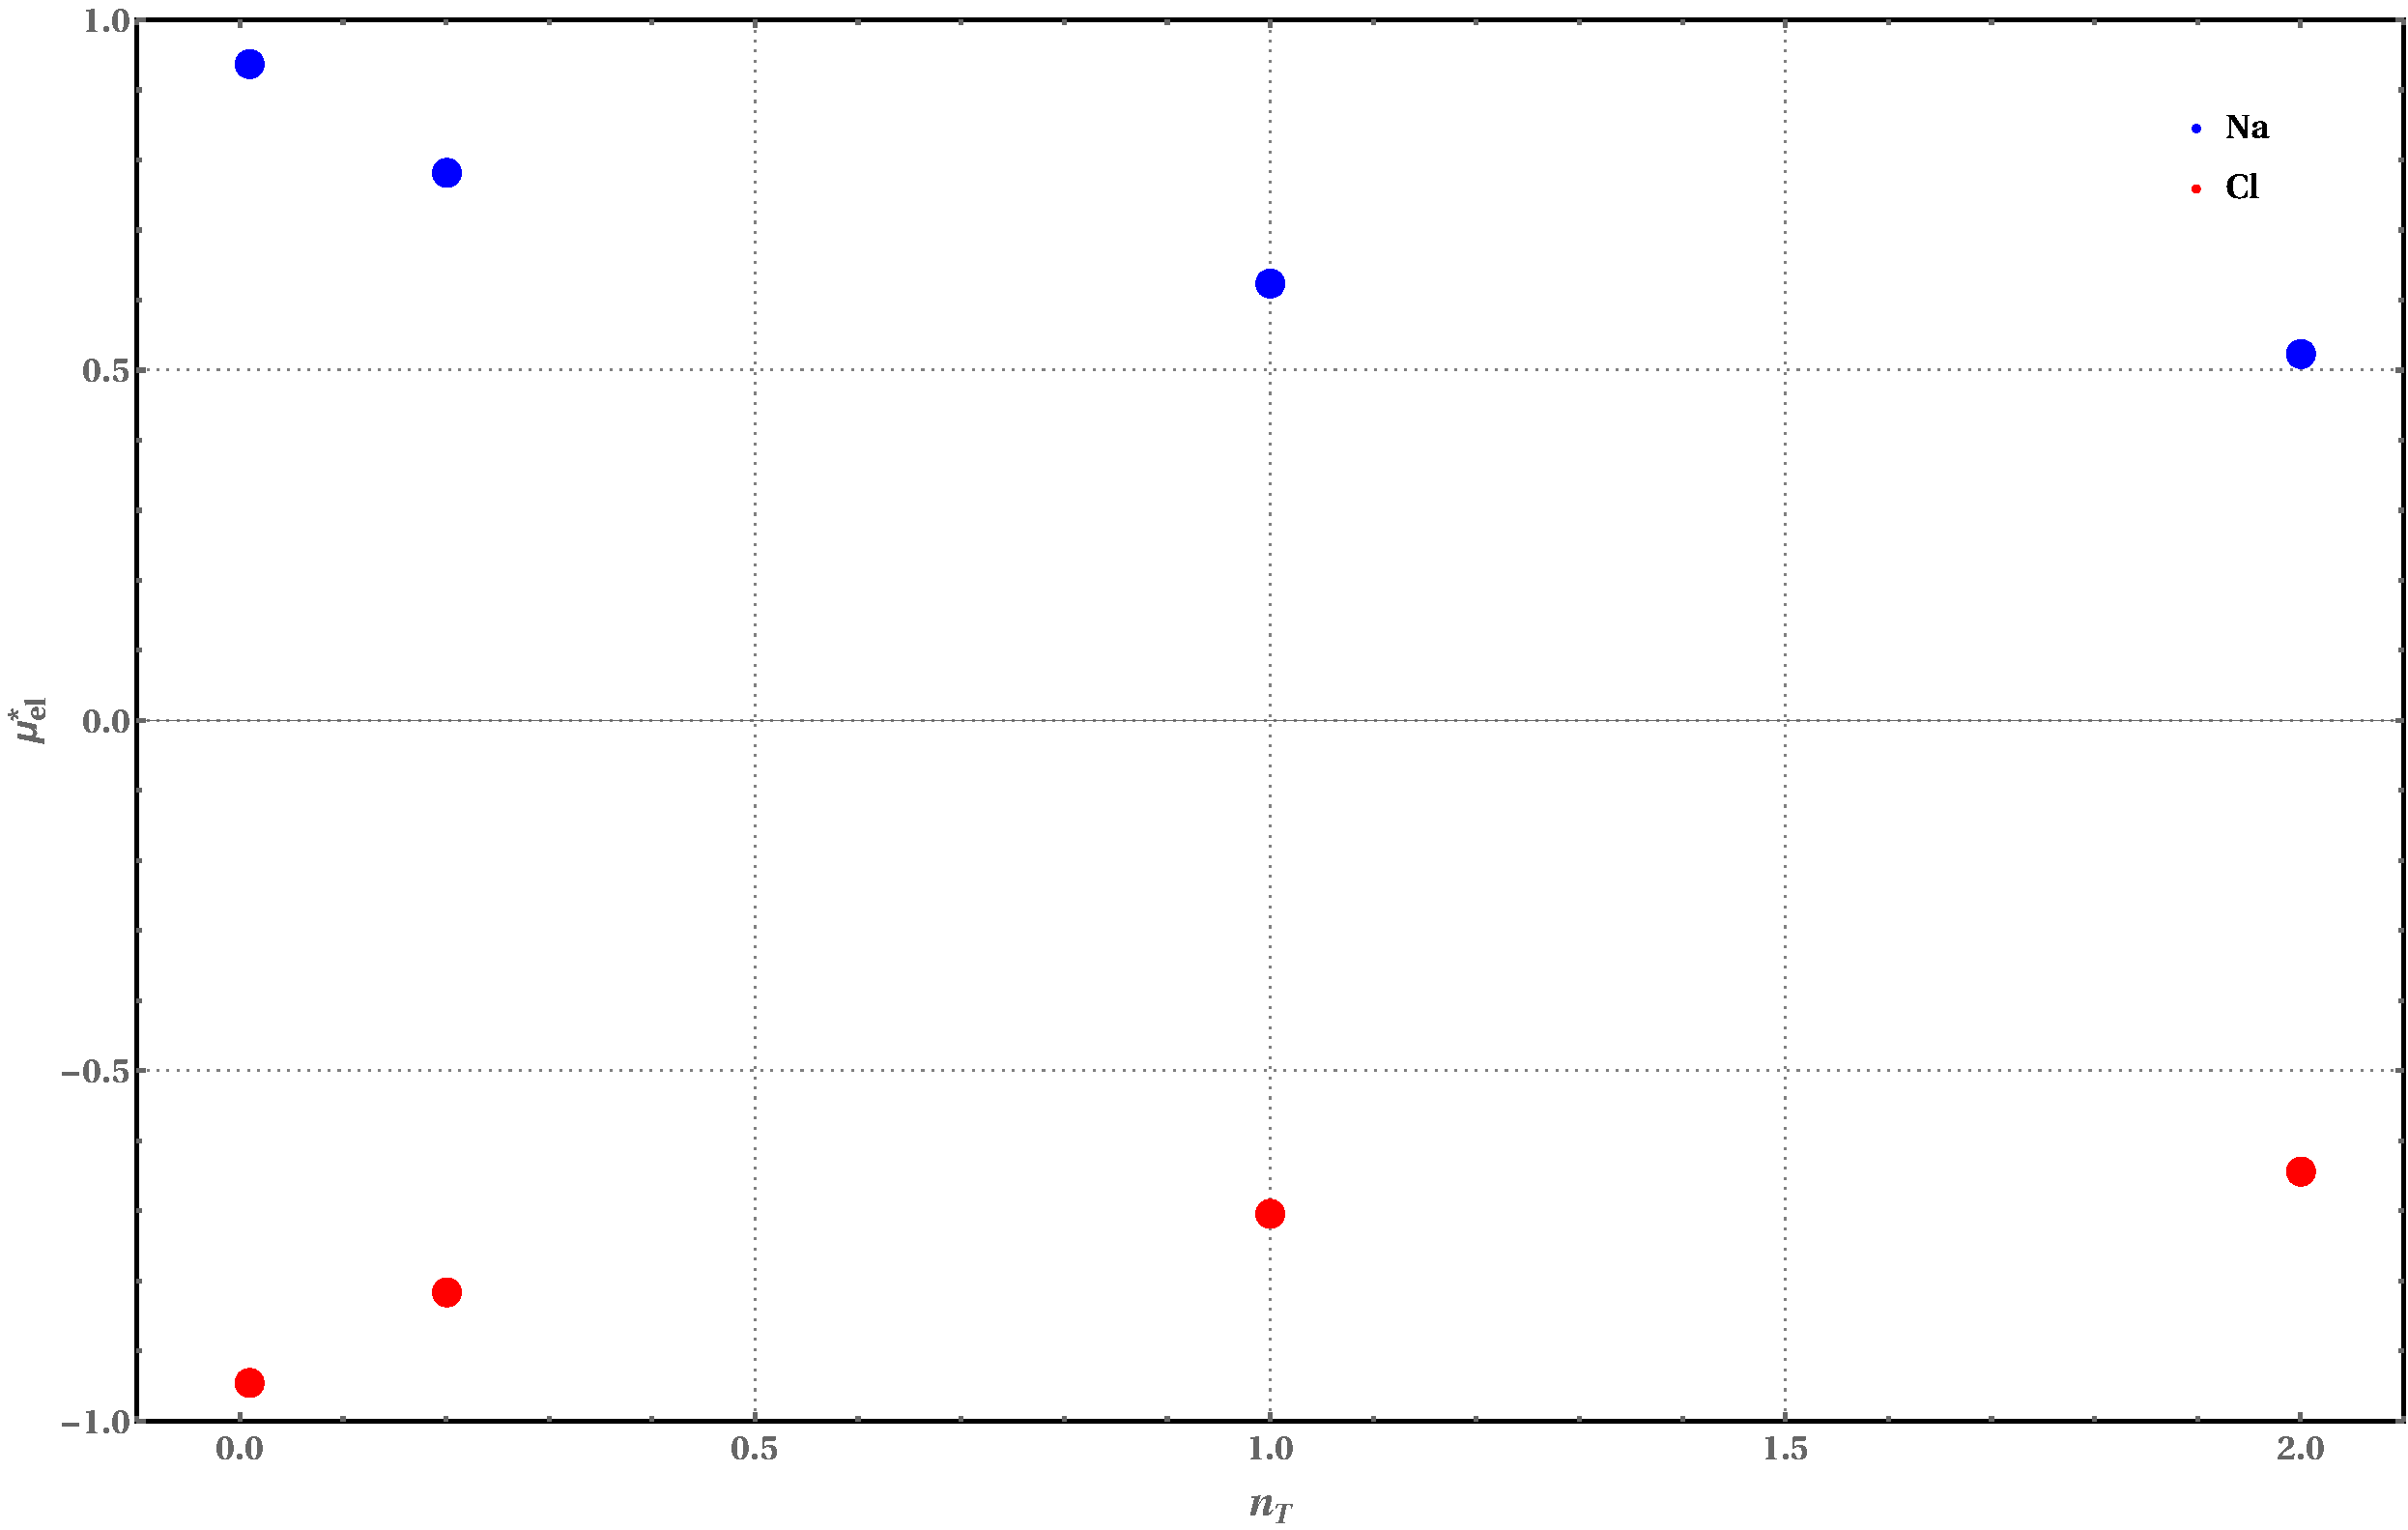
\includegraphics [width=0.95\columnwidth] {Resultados_Movility_NaCl.pdf}
\par}
{\centering
\textbf{Figure 3.} Mobility as function of the density.
\par}
\end{minipage}}
\end{center}
}
%----------------------------------------------------------------------------------------
%	CALIBRATION
%----------------------------------------------------------------------------------------
\headerbox{\small MCT-HI\'s and HNC Approximation}{name=calibration,column=0,row=0,span=1,below=abstract}
{
\begin{center}
\noindent\shadowbox{\begin{minipage}[t]{1\textwidth - 2\fboxsep - 2\fboxrule - 2\shadowsize}%
{\centering
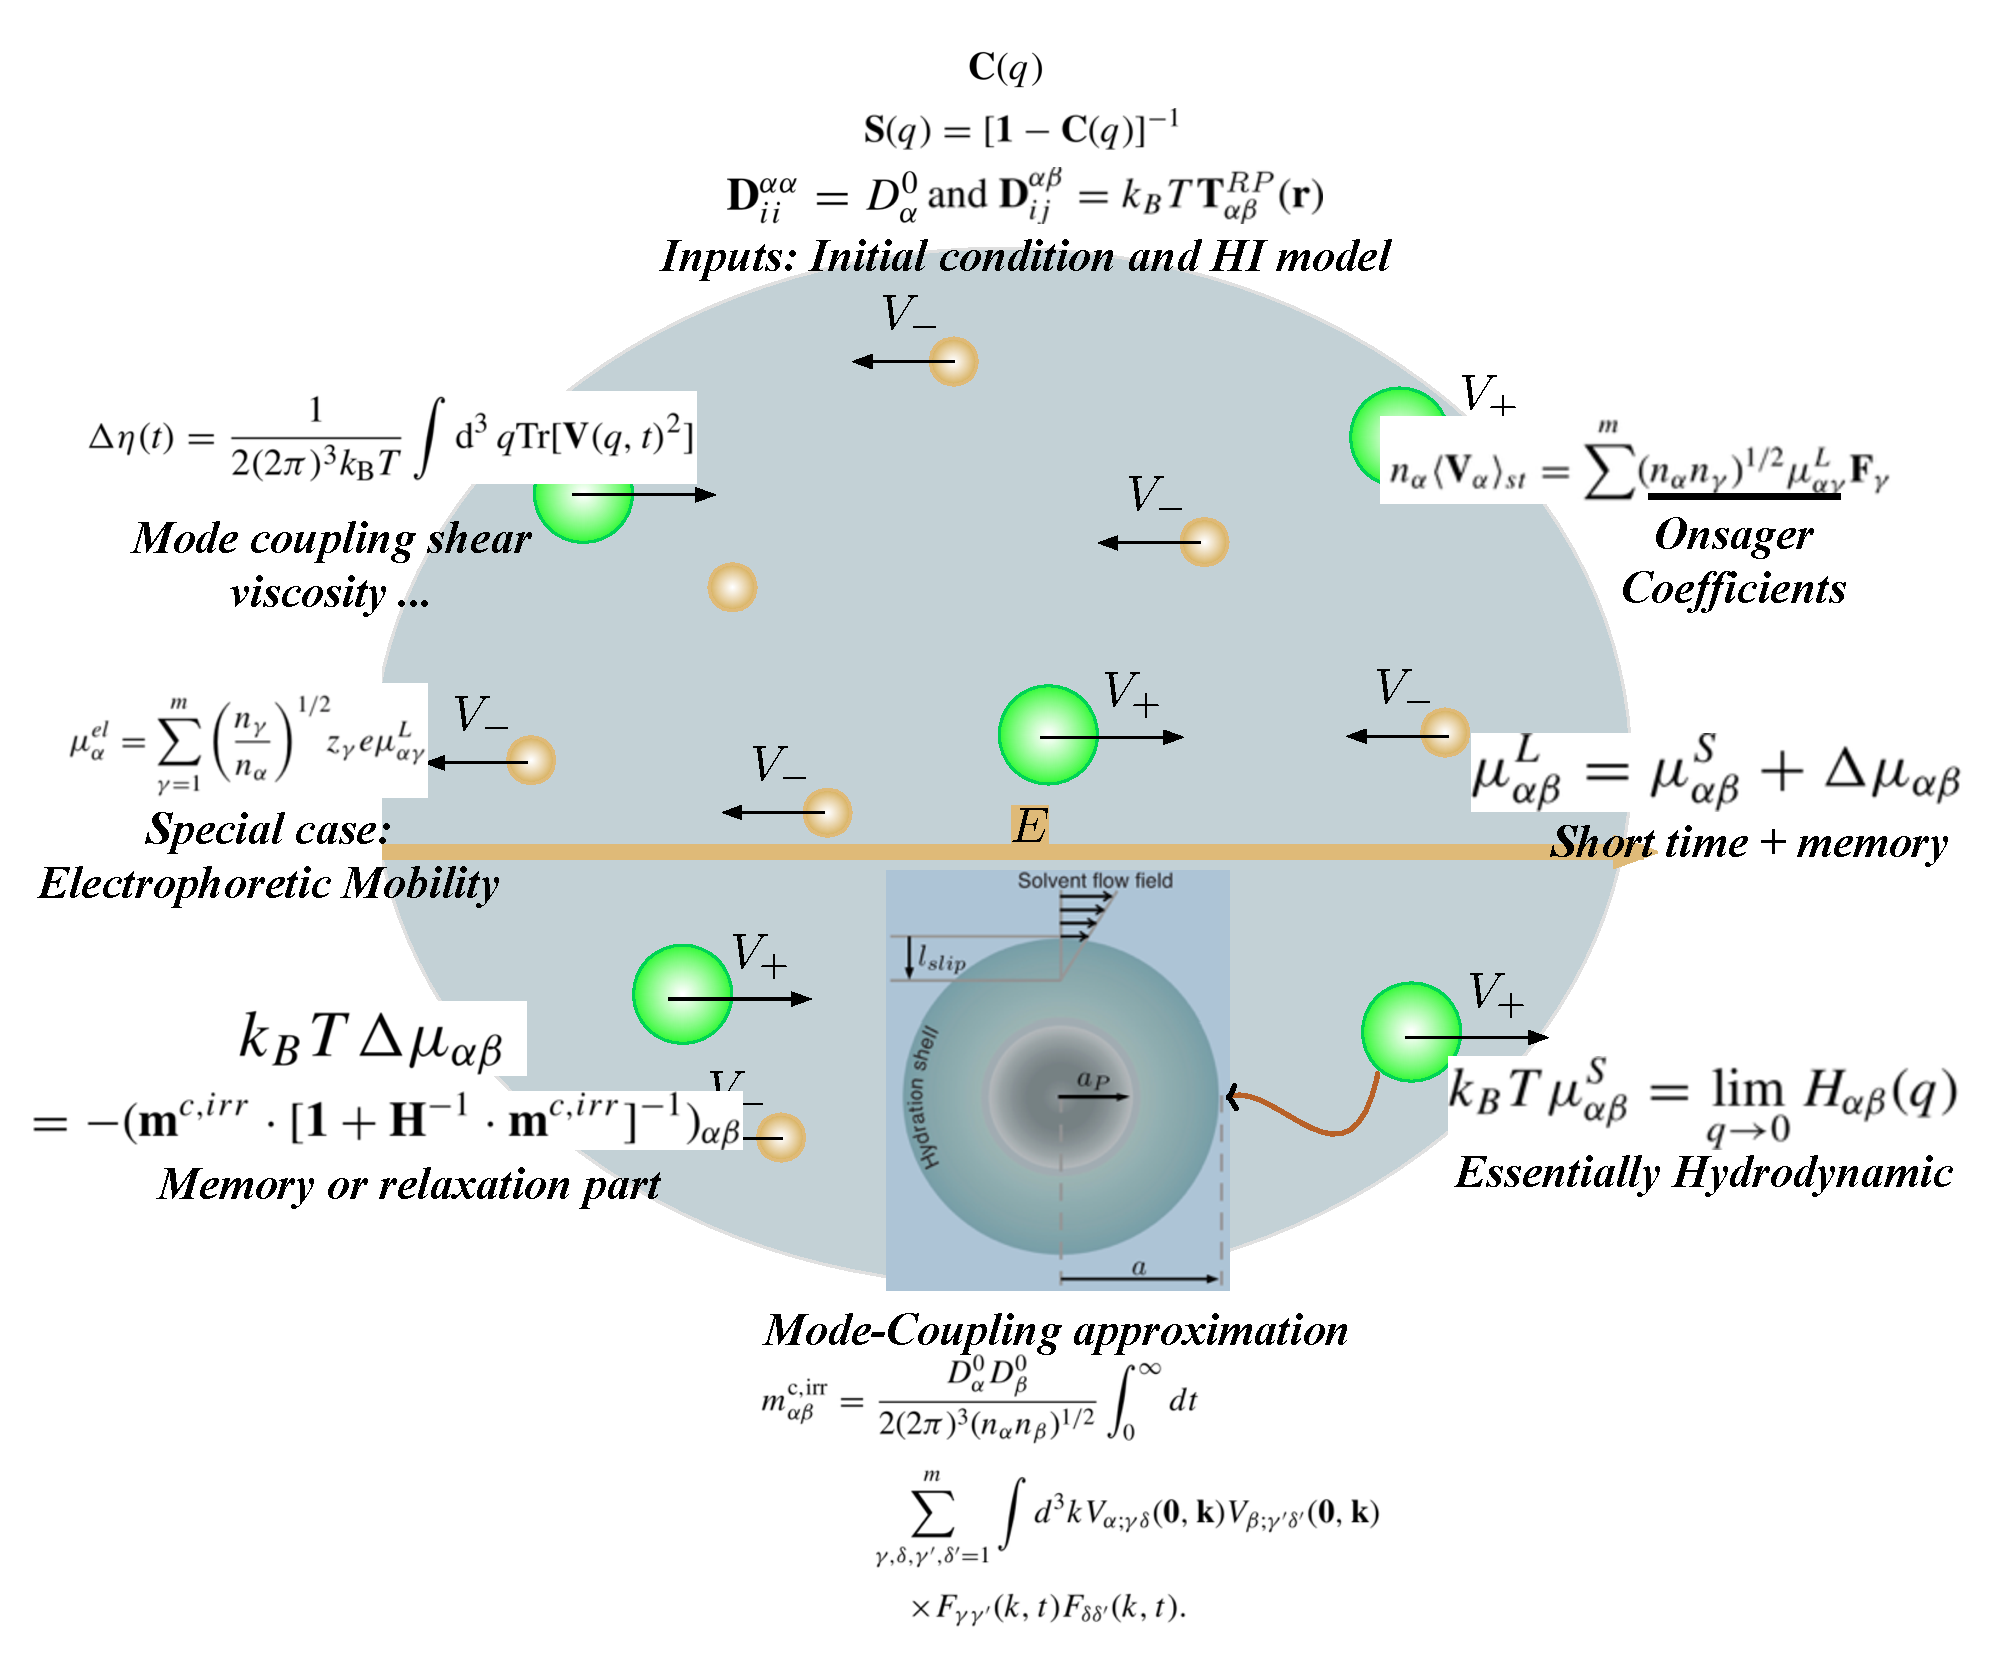
\includegraphics [width=0.70\columnwidth] {Fig1IMA.pdf}
\par}
{\centering
\textbf{Figure 1.} MCT-HI's Theoretical Framework.
\par}
\end{minipage}}
\end{center}
\\
\textbf{HNC Approximation}
\\
The hypernetted chain (HNC) approximation is based on the Ornstein-Zernike (OZ) equation.
For multi-component mixtures, the OZ equation reads $$h_{ij}(r)=c_{ij}+\sum_{k}\rho_{k}\int h_{ik}(|\boldsymbol{r}-\boldsymbol{r}'|)c_{kj}(\boldsymbol{r}')d\boldsymbol{r}'$$ where $h(r)$ and $c(r)$ are the total and direct correlation functions, respectively. \\
\\
A general closure relation between $h(r)$ and $c(r)$ for the OZ
equation is $$\log\left[h_{ij}(r)+1\right]=-\beta u_{ij}(r)+h_{ij}(r)-c_{ij}(r)+\mathcal{B}_{ij}(r)$$ 
$B_{ij}(r)$ is in literature known as the ''bridge grap'' and cannot be written as a closed form function of the distribution functions $h(r)$ and $c(r)$.
\begin{center}
\noindent\shadowbox{\begin{minipage}[t]{1\textwidth - 2\fboxsep - 2\fboxrule - 2\shadowsize}%
{\centering
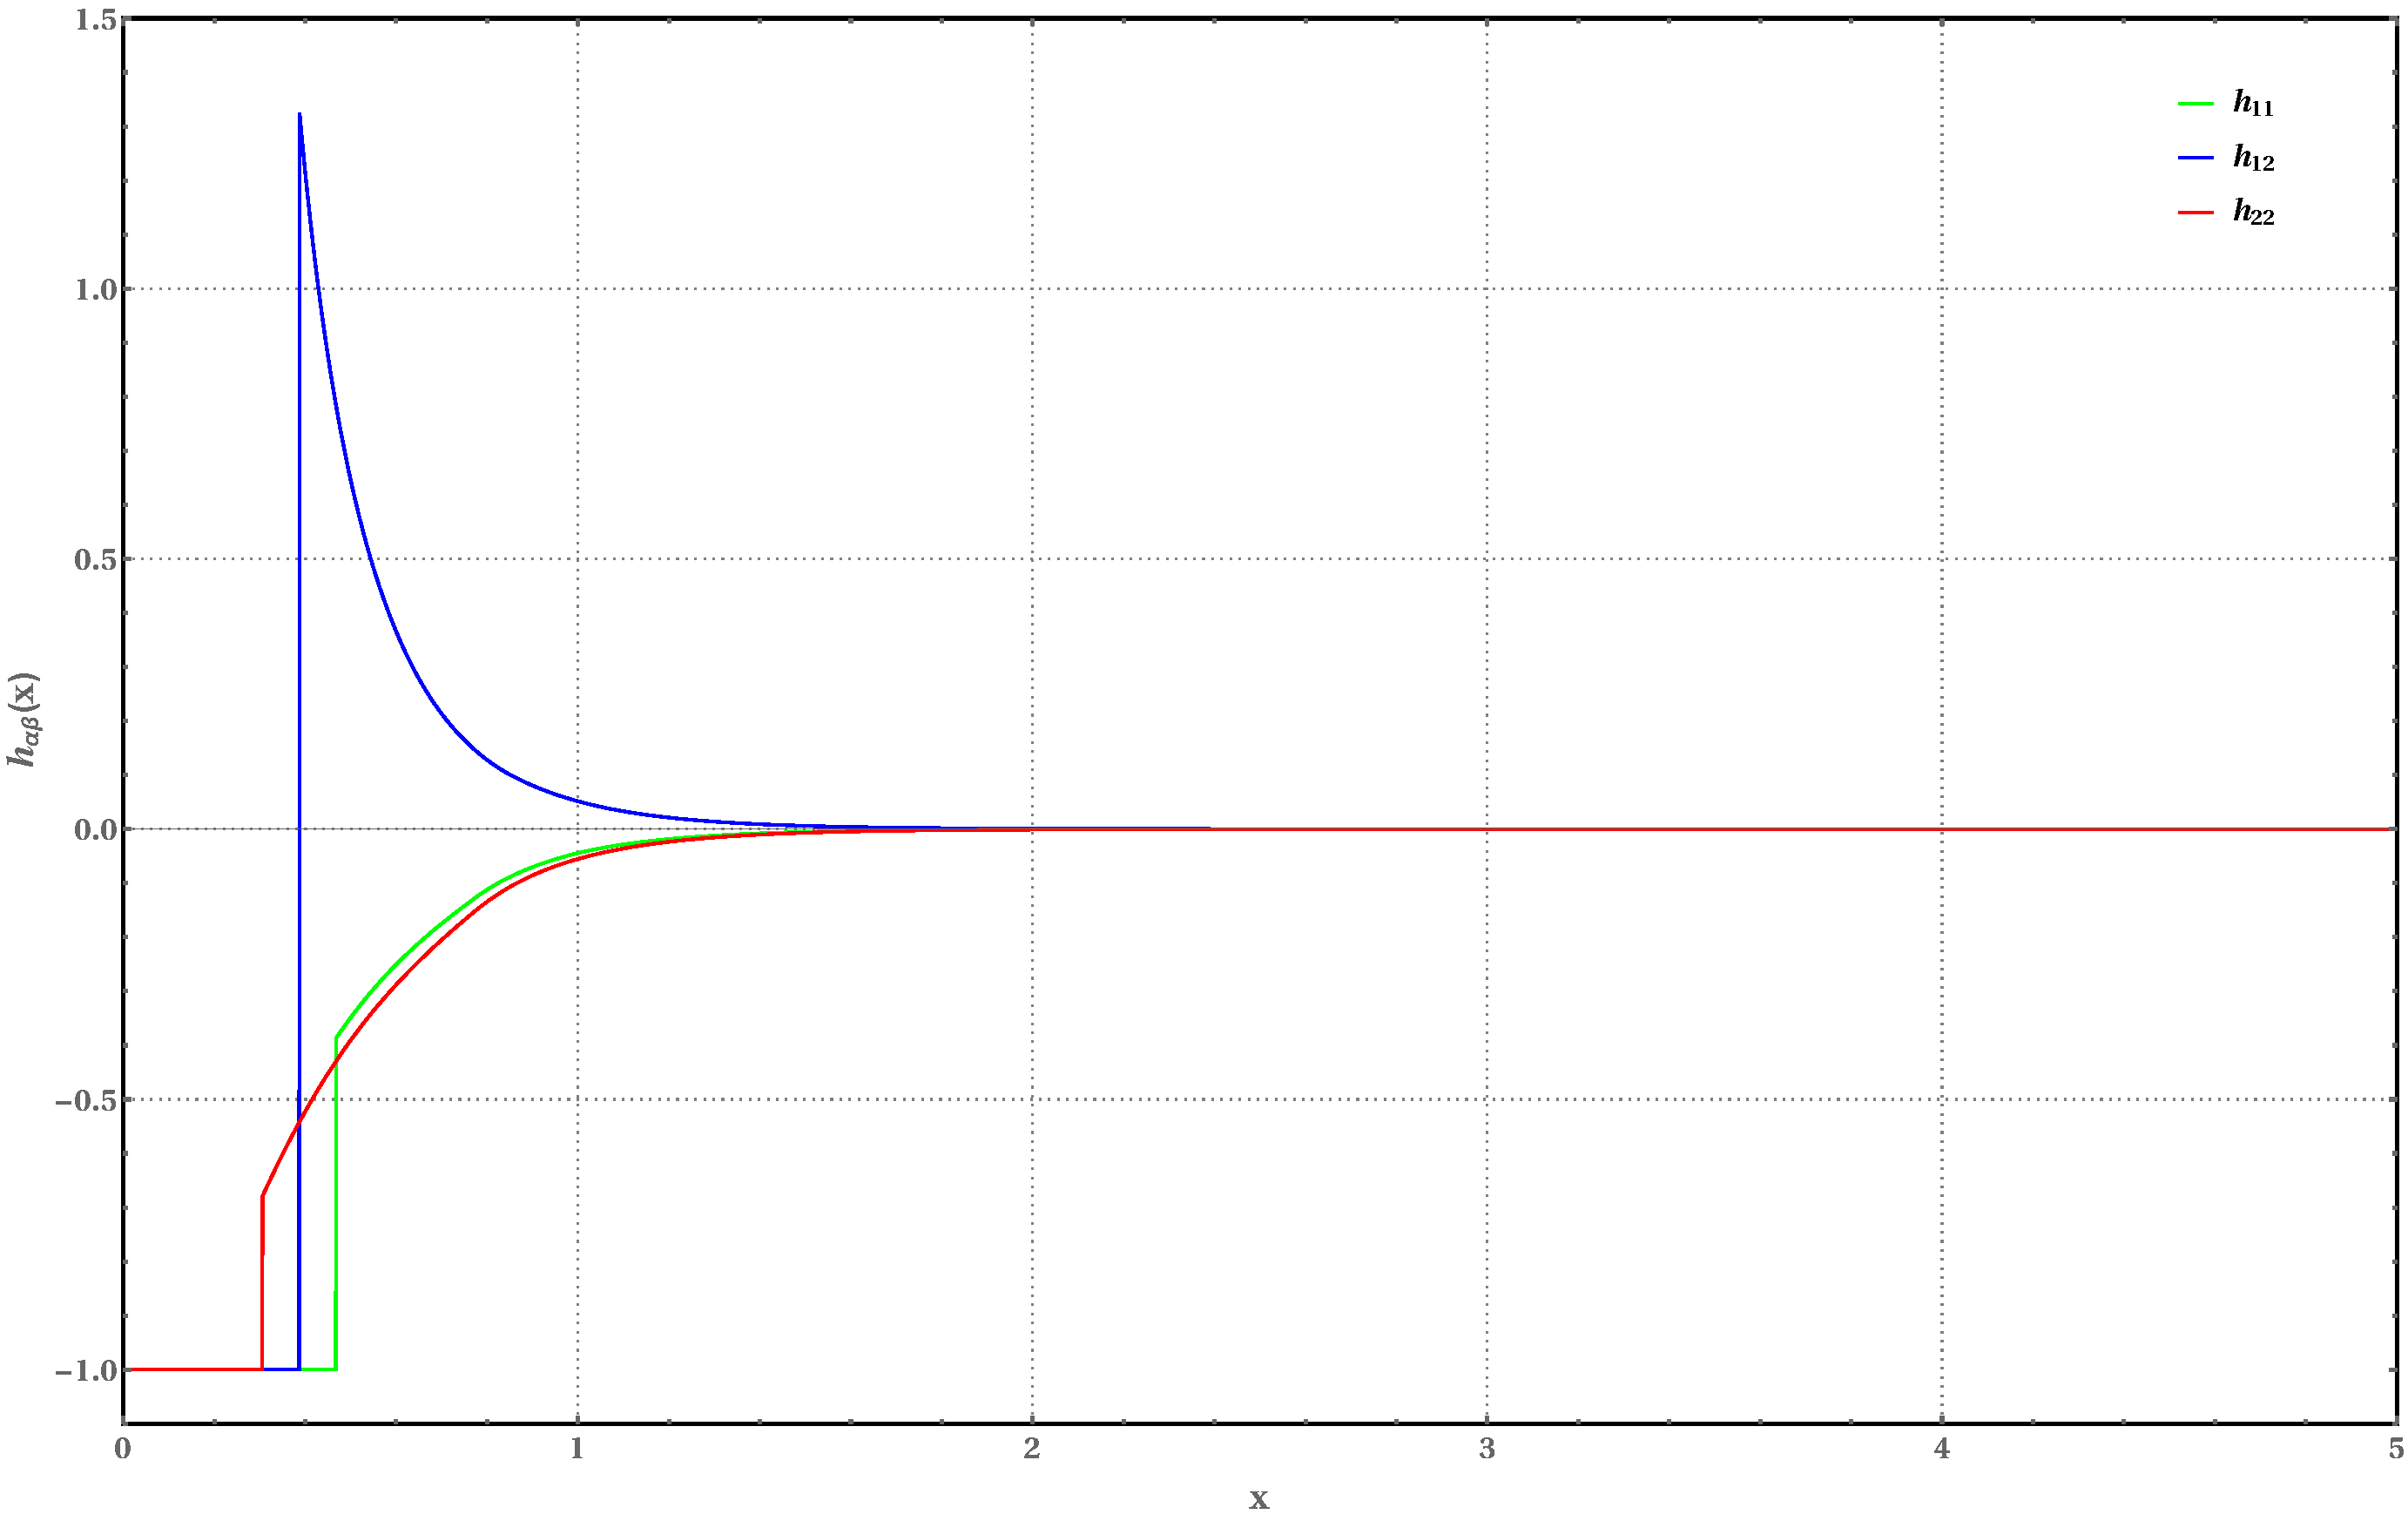
\includegraphics [width=0.95\columnwidth] {NaCl_n1.pdf}
\par}
{\centering
\textbf{Figure 2.} Correlation function for NaCl to $1[M]$.
\par}
\end{minipage}}
\end{center}
}

%----------------------------------------------------------------------------------------
%	MIXER vs. SAMPLERS
%----------------------------------------------------------------------------------------
\headerbox{\small \small \small Conductivity MCT-HI's vs. Experiment}{name=receiver,span=1,column=1,row=1, below=instruments}{\begin{center}
\noindent\shadowbox{\begin{minipage}[t]{1\textwidth - 2\fboxsep - 2\fboxrule - 2\shadowsize}%
{\centering
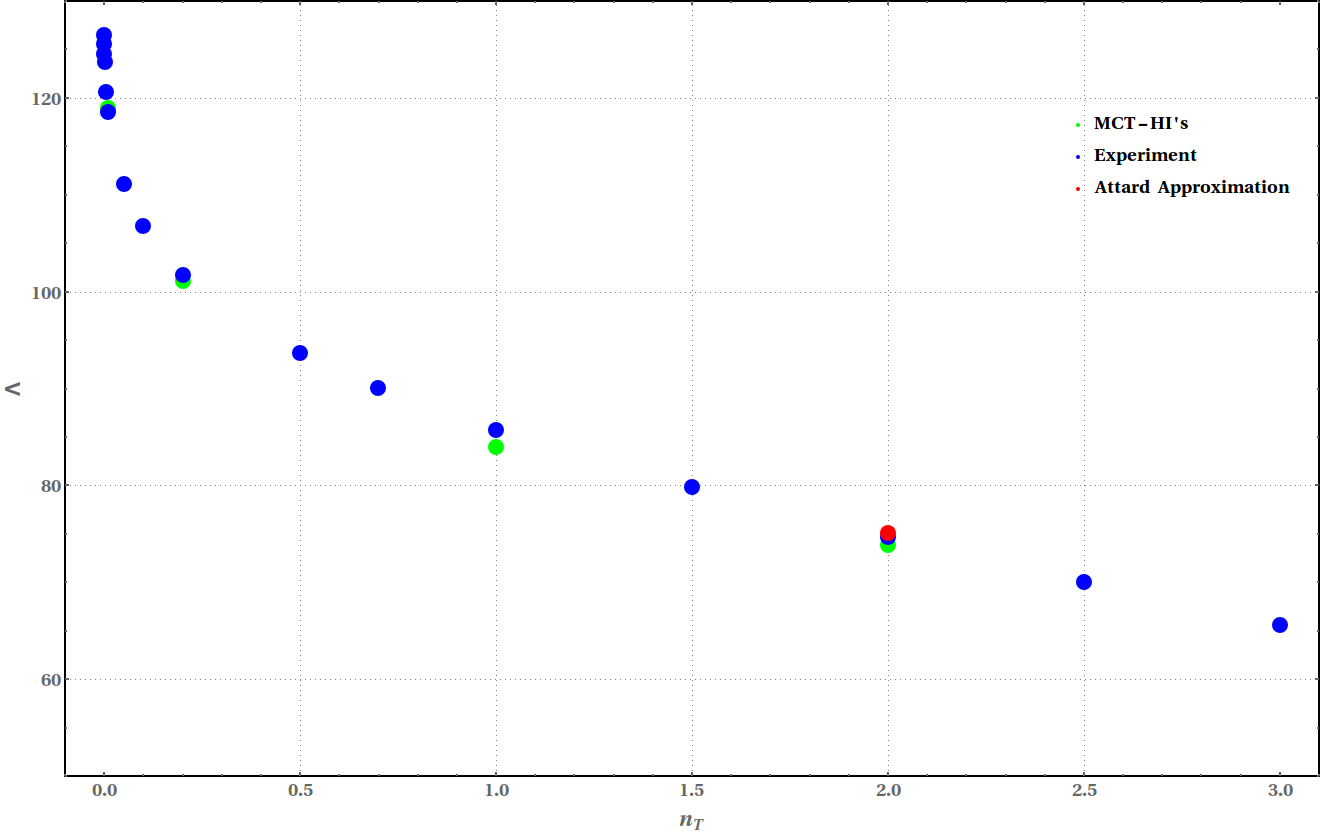
\includegraphics [width=0.95\columnwidth] {Resultados_Graficas_NaCl.png}
\par}
{\centering
\textbf{Figure 3.} Conductivity for different salts.
\par}
\end{minipage}}
\end{center}

}
%----------------------------------------------------------------------------------------
%	CONCLUSION
%----------------------------------------------------------------------------------------
\headerbox{\small References}{name=references,column=1,below=receiver,above=bottom}
{
%\bibliographystyle{plane}
%\bibliography{biblio}
%\begin{thebibliography}{8}
%\small{
[1] Contreras Aburto C. and Naegele G., J. Chem. Phys. 139, 134109 (2013).\\

[2] Contreras Aburto C. and Naegele G., J. Chem. Phys. 139, 134110 (2013).\\

[3] D. G. Miller, J. Phys. Chem. 70, 2639 (1966).\\

[4] M. Heinen, E. Allahyarov, H. Lowen. J. Comput. Chem. 2014, 35, 275-289.
}
%\end{thebibliography}
%}

%----------------------------------------------------------------------------------------
%	REFERENCES
%----------------------------------------------------------------------------------------
%\headerbox{References}{name=references,column=1,below=conclusion,span=2}{

%}
%----------------------------------------------------------------------------------------
%	ACKNOWLEDGEMENTS
%----------------------------------------------------------------------------------------
\headerbox{\small Agradecimientos}{name=acknowledgements,column=0,row=2,below=calibration, above=bottom}{
\small{Al apoyo otorgado a trav\'es del proyecto F-PROMEP-38/Rev-04 y a PFCE 2018}
} 
\end{poster}
\end{document}